\chapter{Literature Overview}\label{chap:lit}
\begin{overview}
  A summary of the mathematical techniques used in this dissertation is given in this chapter.
  Special attention is given to convex geometry and the properties of these sets.

  To place the Operability Index in context, process operability and methods to quantify it are reviewed.
  Finally, the Operability Index is defined and its application to model predictive controllers and their constraints are discussed.  
\end{overview}

\section{Mathematical Preliminaries}
\subsection{Convex Geometry}
\subsubsection{Nomenclature}
The following nomenclature is reviewed and used throughout this document \citep[487]{bayerlee}:
\begin{itemize}
\item polytope - the intersection of closed half-spaces in $\mathbb{R}^n$.
A polytope of $n$ dimensions will simply be referred to as an $n$-polytope.
\item vertex - a 0-dimensional face of an \npoly.
\item facet - an $(n-1)$-dimensional face of an \npoly.
\end{itemize}%
\nomenclature[a]{$n$}{Number of dimensions (variables)}%

\subsubsection{Half-space geometry}\label{sec:hgeometry}
A half-space is defined as the section of an $n$-dimensional space lying on one side of an ($n-1$)-dimensional hyperplane \citep[1282]{crcmaths}.
Linear constraints are equivalent to half-spaces in $\mathbb{R}^n$ in both their mathematical description and meaning.
From this we can conclude that all polytopes generated by linear constraints (half-spaces) are convex, as they have supporting hyperplanes at each boundary point \citep[21]{manilev}.
From this it also follows that the intersection of such convex polytopes will be convex.
This is due to the resulting intersection being merely a subset of the half-spaces defining the two intersecting polytopes.

The problem of degeneracy can occur when constructing polytopes from half-spaces.
Degeneracy is defined when objects ``change their nature to belong to another, usually simpler, class'' \citep[688]{crcmaths}.
The degeneracy of polytopes is important for the purposes of this dissertation.
When the number of half-spaces used to construct a polytope is more than the final number of facets on the resulting closed polytope, the polytope is classified as degenerate.

\subsubsection{Convex hull and vertex enumeration}
The convex hull or facet enumeration is used extensively for calculations in this project.
It is defined as the smallest convex set containing $P$ if $P$ is a set of points ($P \subseteq \mathbb{R}^n$) \citep[74]{wenger}.
In this project, $P$ is generated from a set of half-spaces and the resulting vertices are the minimum vertex description of $P$.
For this reason the convex hull of $P$ and the half-spaces used to generate $P$ are equivalent.

The opposite of facet enumeration is vertex enumeration, where a set of half-spaces are transformed to the vertices of $P$.
A primal-dual method can be implemented to solve this problem.
The full mathematical formulation of the primal-dual algorithm is omitted from this document.
\citet[636-639]{primaldual1} and \citet{primaldual2} can be consulted for the full formulation. 

\subsubsection{Linear transformations}
Define $X$ and $Y$ as finite-dimensional sets with bases $(x_1,\dots,x_n)$ and $(y_1,\dots,y_m)$ respectively.
For the linear transformation $\phi : X \to Y$, the following holds:
\begin{equation}
  \label{eq:lintrans}
  \phi(y_i) = \alpha_{i1}x_i+\cdots+\alpha_{in}x_n \text{~~~for~} i = 1, \dots, m
\end{equation}
The scalars $(\alpha_{ij})_{i=1,\dots,n;~j=1,\dots,m}$ can be written as
\begin{equation}
  \bpm
    \alpha_{11} &\cdots &\cdots &\alpha_{1n} \\
    \alpha_{21} &\cdots &\cdots &\alpha_{2n} \\
    \cdots     &\cdots &\cdots &\cdots \\
    \alpha_{m1} &\cdots &\cdots &\alpha_{mn} \\
  \epm \notag
\end{equation}
which is referred to as the matrix of $\phi$ \citep[48-49,~166]{leung}.

Equation~\ref{eq:lintrans} is equivalent to the result of the following matrix multiplication
\begin{equation}
  \label{eq:matmult}
  \Phi X = Y
\end{equation}
where $\Phi$ is the matrix of $\phi$.
Equation~\ref{eq:matmult} confirms that matrix multiplication is indeed a linear transformation.

\subsection{Process models}
The mathematical description of process models and specifically the space transformations those lead to are of importance.

\subsubsection{Linear steady-state}
The steady-state model of a linear system is the gain-matrix.
This is simply a matrix of constants in $\mathbb{R}$.
Models like these allow for matrix algebra when transforming between spaces, e.g. a matrix multiplication of the input space and the process model has the output space as result.

The transformation obtained for linear models are conformal mappings.
This is defined as a mapping that preserves local angles and has a non-zero differential at every point \citep[514]{crcmaths}.
Being conformal, the surface (or boundary) of the input space (a polytope) maps directly to the surface of the output space.
For this reason, the constraints specifying a space can be used to generate the corresponding space with full mathematical rigour.

\subsubsection{Non-linear models}
The mapping of spaces via non-linear models is not guaranteed to be conformal.
Therefore, the statement that boundaries map to boundaries in their corresponding spaces, cannot be made.

A practical example of this is illustrated by \citet{opidealrx}, for a vinyl acetate reactor where a set of inputs map to the same point in the output space.
In this case, the phenomena of input multiplicities is ascribed to a rank deficiency of the Jacobian matrix of the process model.


\section{Process Operability}
The method of constraint handling presented in this document, is largely derived from work done by Georgakis and colleagues, in particular \citet{vinsonphd}, \citet{vinsonartoi}, \citet{limaphd}, \citet{opconproc} and \citet{opidealrx}. 
To place the Operability Index of \citet{vinsonphd} (defined in section~\ref{sec:oi}) in context, a short overview of process operability and the most common process operability techniques is presented below.

\subsection{Overview}
Process operability is defined as ``the ease with which a process can be operated and controlled'' \citep[778]{marlin}.
Process operability is an ongoing field of study with many of the methods available being only qualitative \citep[164]{skogestad}. 
A distinction is made between steady-state (input and output relationships at steady-state only) and dynamic operability methods.

\subsubsection{Steady-state operability measures}
The relative gain array (RGA) is one of the most used operability measures \citep[576]{luyben} and relates input and output interactivity.
Each element in the RGA ($\beta_{ij}$) is defined as the ratio of the steady-state gain ratios between input, $i$, and output, $j$, when all other inputs and outputs are constant.
\citet{artrdg} defined the RDG, which expanded on the RGA to include the effect of disturbances. 
Considering only the magnitudes of RGA elements can be misleading \citep[87]{skogestad}, as seemingly favourable pairings can be unfavourable due to the phase.
Therefore, both the magnitude and the phase need to be considered or, alternatively, norms such as the RGA-number can be used.


The Niederlinski index is another measure that only uses steady-state gains of the process model \citep[572-573]{luyben}.
Positive values of the Niederlinski index can correspond to unstable pairings and are therefore inconclusive.
For this reason, the index is considered necessary but not sufficient for stability \citep[445]{skogestad}.

Singular value decomposition stems from the use of eigenvalues as an operability measure. 
The use of singular values are preferred as eigenvalues are a poor
measure of gain and can often be misleading \citep[75]{skogestad}.
Maximum and minimum singular values are mostly used to select controlled variables but can also be used as a performance measure along with the condition number \citepp{596}{luyben}{80-82}{skogestad}.

\subsubsection{Dynamic operability measures}
The RGA can be expanded to contain frequency-dependant terms and is often referred to as the dynamic relative gain array (DRGA) \citep[637]{marlin}. 
The RDG \citep{artrdg} can be expanded in a similar way to include frequency-dependant terms.

Nyquist array methods as defined by Rosenbrock, as quoted by \citet[92]{skogestad}, are an extension of the SISO Nyquist stability criteria that include frequency dynamics. 
The two methods developed are the direct Nyquist array and the inverse Nyquist array. 
When used in conjunction with Gershgorin bands, conditions for overall stability can be derived \citep[440]{skogestad}.

\citet{vinsonphd} lists other dynamic operability measures which rely on the choice of a controller type. Further shortcomings of the above mentioned operability measures are also discussed in that text. 

\subsection{Operability Index}\label{sec:oi}
The Operability Index was defined by \citet{vinsonphd} as a measure of steady-state process operability. 
Constraint interdependence is used as the basis of this index. 
Further work by \citet{limaphd} expanded this index to cover non-square systems and some application to dynamic systems.%
\nomenclature[ba]{OI}{Operability Index}%

\subsubsection{Definitions}
The Operability Index focuses on input-output relationships rather the system's dynamic states \citep{vinsonphd}. 
Input and output values are defined by spaces (in $\mathbb{R}^n$ and $\mathbb{R}^m$, with $n$ the number of inputs and $m$ the number of outputs). 
These spaces are the feasible regions which are bounded by the inequalities describing the ranges of the inputs or outputs. 
The following spaces are of interest:%
\nomenclature[a]{$u$}{System inputs}%
\nomenclature[a]{$x$}{System states}%
\nomenclature[a]{$y$}{System outputs}%

\begin{description}
  \item [Available Input Space (AIS);] the set of attainable values of the process inputs. 
    The limits on these values are based on both physical limits (e.g.     valve openings) or process design values (e.g. flow-rates or temperatures). 
Figure~\ref{fig:sampleaisaos} illustrates an AIS for two variables ($u_1, u_2$) bounded by simple high and low limits.%
\nomenclature[ba]{AIS}{Available Input Space}%
  \item [Achievable Output Space (AOS);] this is the set of values which the process outputs can obtain, given the AIS. 
The AIS maps to the AOS by means of a process model, $G$. 
Therefore, a point $u$ in the AIS corresponds to a point $y$ in the AOS via $y=G(u)$. 
Examples of AOSs for linear and non-linear models are shown in figure~\ref{fig:sampleaisaos}.%
\nomenclature[a]{$G$}{Process model}%
\nomenclature[ba]{AOS}{Available Output Space}%
  \item [Desired Output Space (DOS);] this represents the desired output values of a process. 
These values are typically based on operational and financial   parameters. 
Figure~\ref{fig:sampledos} shows a sample DOS for a two output    system along with a sample AOS.%
\nomenclature[ba]{DOS}{Desired Output Space}%
  \item [Expected Disturbance Space (EDS);] all the values of the expected disturbances to the system. 
These values are translated back to the input space by means of the disturbance model, $G_d$.%
\nomenclature[ba]{EDS}{Expected Disturbance Space}%
  \item [Desired Input Space (DIS);] in the same manner that the AIS maps to the AOS, the DIS represents combined reverse mappings of the DOS and EDS.
The DIS is calculated as the inputs, $u$, that satisfy the model, i.e. $y=G(u,d)$ (with $y$ and $d$ from the DOS and EDS respectively).
Figure~\ref{fig:sampledis} shows this combined translation.%
\nomenclature[a]{$d$}{System disturbance}%
\nomenclature[ba]{DIS}{Desired Input Space}%
\end{description}

\begin{figure}[htbp]
  \centering
%  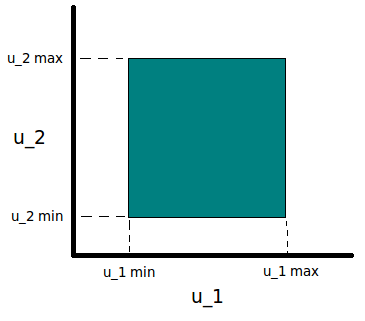
\includegraphics[width=8cm]{graph/sample_ais}
  \scalebox{1}{% Graphic for TeX using PGF
% Title: /home/andre/GIT Repos/AHCampher_thesis/diagrams/sampleaisaos.dia
% Creator: Dia v0.97.1
% CreationDate: Thu Jan  6 14:07:33 2011
% For: andre
% \usepackage{tikz}
% The following commands are not supported in PSTricks at present
% We define them conditionally, so when they are implemented,
% this pgf file will use them.
\ifx\du\undefined
  \newlength{\du}
\fi
\setlength{\du}{15\unitlength}
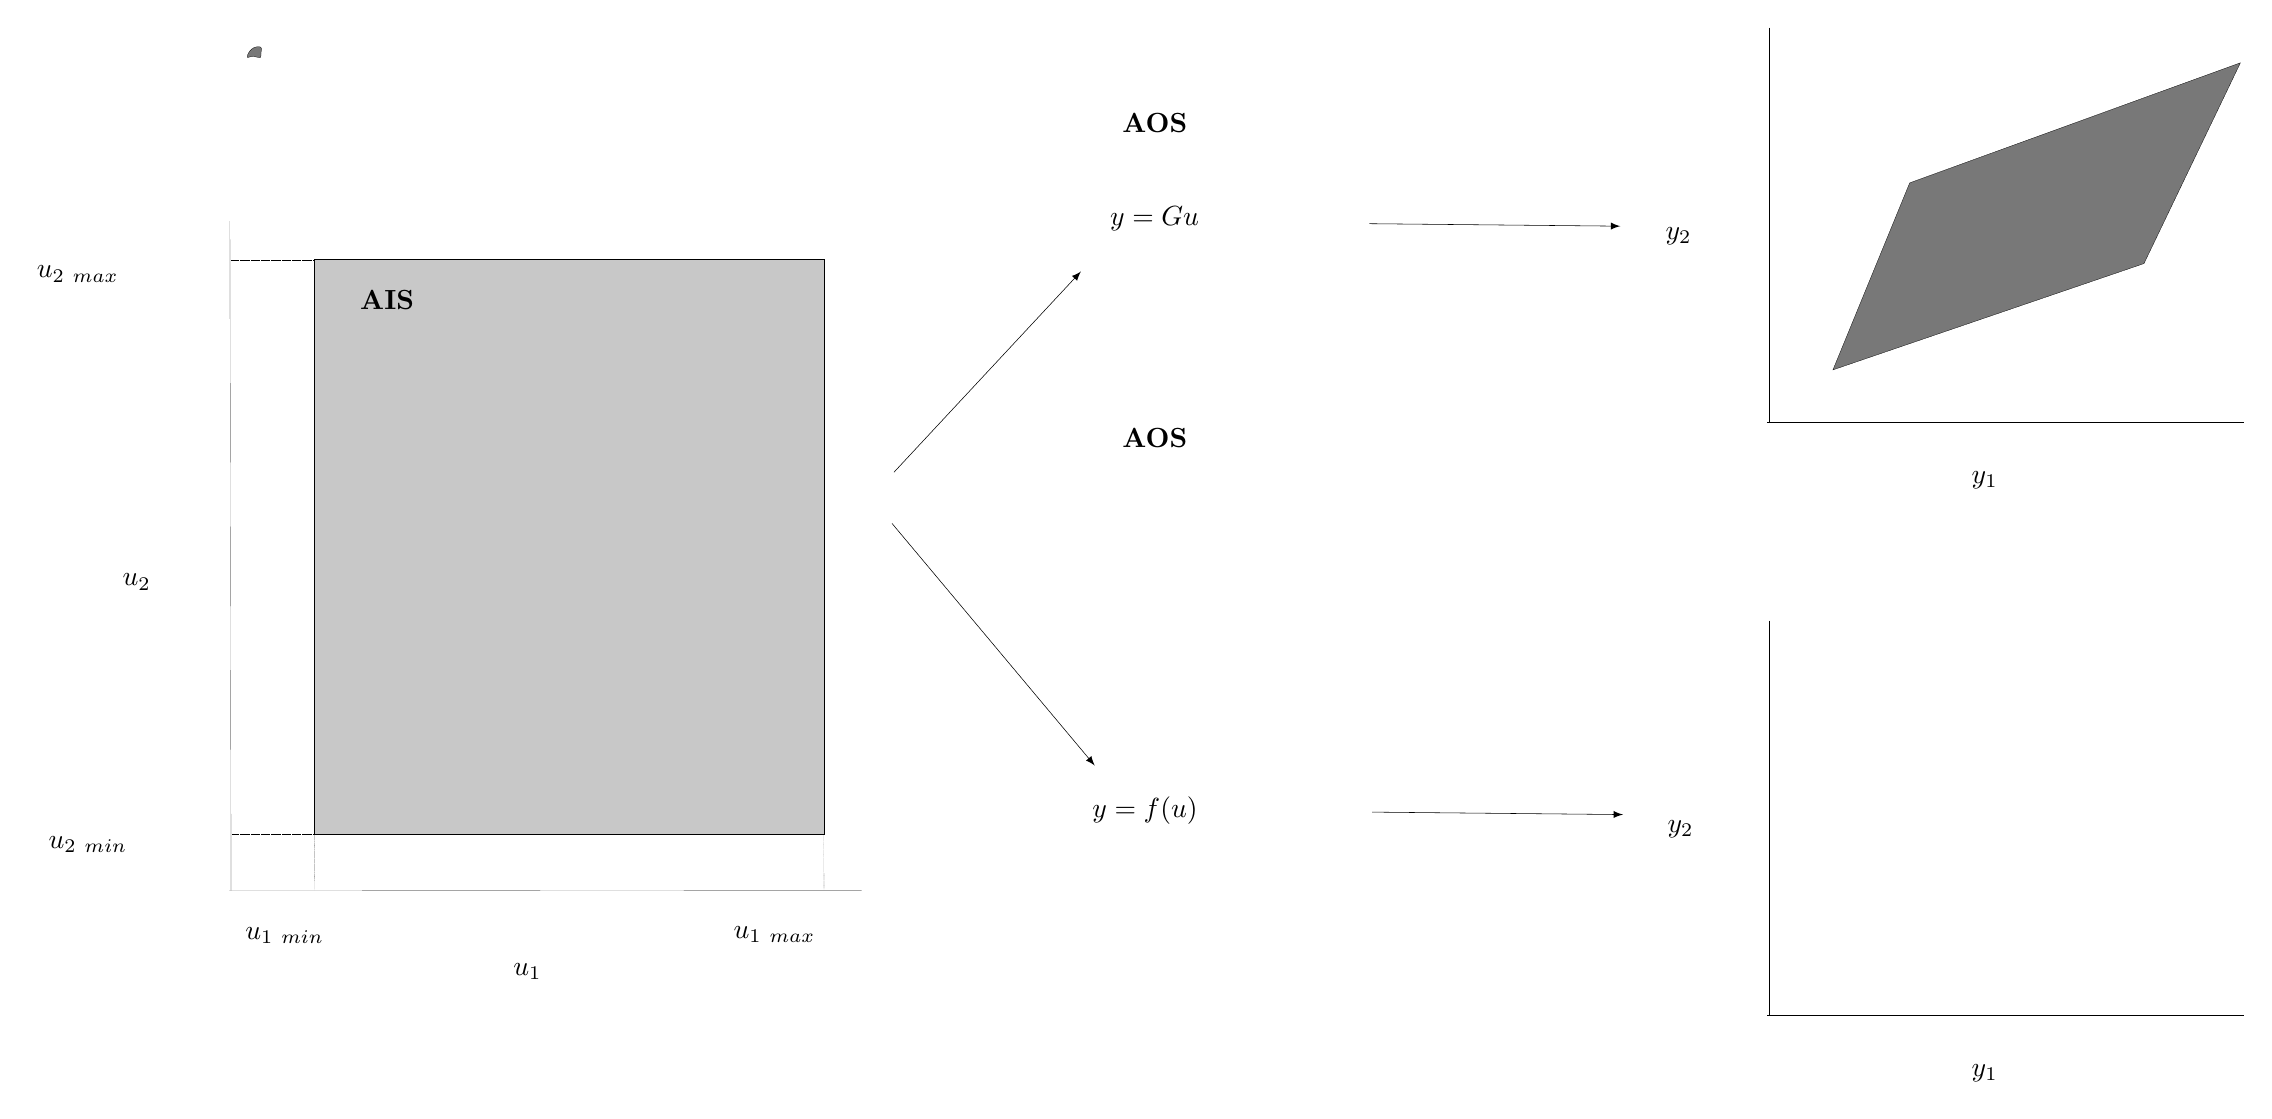
\begin{tikzpicture}
\pgftransformxscale{1.000000}
\pgftransformyscale{-1.000000}
\definecolor{dialinecolor}{rgb}{0.000000, 0.000000, 0.000000}
\pgfsetstrokecolor{dialinecolor}
\definecolor{dialinecolor}{rgb}{1.000000, 1.000000, 1.000000}
\pgfsetfillcolor{dialinecolor}
\pgfsetlinewidth{0.100000\du}
\pgfsetdash{}{0pt}
\pgfsetdash{}{0pt}
\pgfsetmiterjoin
\definecolor{dialinecolor}{rgb}{0.784314, 0.784314, 0.784314}
\pgfsetfillcolor{dialinecolor}
\fill (1.574384\du,2.981260\du)--(1.574384\du,10.281260\du)--(8.047075\du,10.281260\du)--(8.047075\du,2.981260\du)--cycle;
\definecolor{dialinecolor}{rgb}{0.000000, 0.000000, 0.000000}
\pgfsetstrokecolor{dialinecolor}
\draw (1.574384\du,2.981260\du)--(1.574384\du,10.281260\du)--(8.047075\du,10.281260\du)--(8.047075\du,2.981260\du)--cycle;
\pgfsetlinewidth{0.050000\du}
\pgfsetdash{}{0pt}
\pgfsetdash{}{0pt}
\pgfsetbuttcap
{
\definecolor{dialinecolor}{rgb}{0.000000, 0.000000, 0.000000}
\pgfsetfillcolor{dialinecolor}
% was here!!!
\definecolor{dialinecolor}{rgb}{0.000000, 0.000000, 0.000000}
\pgfsetstrokecolor{dialinecolor}
\draw (0.503325\du,2.493750\du)--(0.518134\du,10.993760\du);
}
\pgfsetlinewidth{0.050000\du}
\pgfsetdash{}{0pt}
\pgfsetdash{}{0pt}
\pgfsetbuttcap
{
\definecolor{dialinecolor}{rgb}{0.000000, 0.000000, 0.000000}
\pgfsetfillcolor{dialinecolor}
% was here!!!
\definecolor{dialinecolor}{rgb}{0.000000, 0.000000, 0.000000}
\pgfsetstrokecolor{dialinecolor}
\draw (8.525166\du,10.989073\du)--(0.492855\du,10.995323\du);
}
\pgfsetlinewidth{0.050000\du}
\pgfsetdash{{1.000000\du}{1.000000\du}}{0\du}
\pgfsetdash{{0.200000\du}{0.200000\du}}{0\du}
\pgfsetbuttcap
{
\definecolor{dialinecolor}{rgb}{0.000000, 0.000000, 0.000000}
\pgfsetfillcolor{dialinecolor}
% was here!!!
\definecolor{dialinecolor}{rgb}{0.000000, 0.000000, 0.000000}
\pgfsetstrokecolor{dialinecolor}
\draw (1.573559\du,10.987510\du)--(1.574384\du,10.281260\du);
}
\pgfsetlinewidth{0.050000\du}
\pgfsetdash{{0.200000\du}{0.200000\du}}{0\du}
\pgfsetdash{{0.200000\du}{0.200000\du}}{0\du}
\pgfsetbuttcap
{
\definecolor{dialinecolor}{rgb}{0.000000, 0.000000, 0.000000}
\pgfsetfillcolor{dialinecolor}
% was here!!!
\definecolor{dialinecolor}{rgb}{0.000000, 0.000000, 0.000000}
\pgfsetstrokecolor{dialinecolor}
\draw (8.047594\du,10.975010\du)--(8.047075\du,10.281260\du);
}
\pgfsetlinewidth{0.050000\du}
\pgfsetdash{{0.200000\du}{0.200000\du}}{0\du}
\pgfsetdash{{0.200000\du}{0.200000\du}}{0\du}
\pgfsetbuttcap
{
\definecolor{dialinecolor}{rgb}{0.000000, 0.000000, 0.000000}
\pgfsetfillcolor{dialinecolor}
% was here!!!
\definecolor{dialinecolor}{rgb}{0.000000, 0.000000, 0.000000}
\pgfsetstrokecolor{dialinecolor}
\draw (1.574384\du,10.281260\du)--(0.526684\du,10.281260\du);
}
\pgfsetlinewidth{0.050000\du}
\pgfsetdash{{0.200000\du}{0.200000\du}}{0\du}
\pgfsetdash{{0.200000\du}{0.200000\du}}{0\du}
\pgfsetbuttcap
{
\definecolor{dialinecolor}{rgb}{0.000000, 0.000000, 0.000000}
\pgfsetfillcolor{dialinecolor}
% was here!!!
\definecolor{dialinecolor}{rgb}{0.000000, 0.000000, 0.000000}
\pgfsetstrokecolor{dialinecolor}
\draw (1.574384\du,2.981260\du)--(0.519417\du,2.981260\du);
}
% setfont left to latex
\definecolor{dialinecolor}{rgb}{0.000000, 0.000000, 0.000000}
\pgfsetstrokecolor{dialinecolor}
\node[anchor=west] at (-0.978316\du,7.075781\du){$u_2$};
% setfont left to latex
\definecolor{dialinecolor}{rgb}{0.000000, 0.000000, 0.000000}
\pgfsetstrokecolor{dialinecolor}
\node[anchor=west] at (3.984184\du,12.025781\du){$u_1$};
% setfont left to latex
\definecolor{dialinecolor}{rgb}{0.000000, 0.000000, 0.000000}
\pgfsetstrokecolor{dialinecolor}
\node[anchor=west] at (-2.065816\du,3.163281\du){$u_{2~max}$};
% setfont left to latex
\definecolor{dialinecolor}{rgb}{0.000000, 0.000000, 0.000000}
\pgfsetstrokecolor{dialinecolor}
\node[anchor=west] at (-1.917066\du,10.410781\du){$u_{2~min}$};
% setfont left to latex
\definecolor{dialinecolor}{rgb}{0.000000, 0.000000, 0.000000}
\pgfsetstrokecolor{dialinecolor}
\node[anchor=west] at (6.781684\du,11.550791\du){$u_{1~max}$};
% setfont left to latex
\definecolor{dialinecolor}{rgb}{0.000000, 0.000000, 0.000000}
\pgfsetstrokecolor{dialinecolor}
\node[anchor=west] at (0.580434\du,11.565791\du){$u_{1~min}$};
\pgfsetlinewidth{0.050000\du}
\pgfsetdash{}{0pt}
\pgfsetdash{}{0pt}
\pgfsetbuttcap
{
\definecolor{dialinecolor}{rgb}{0.000000, 0.000000, 0.000000}
\pgfsetfillcolor{dialinecolor}
% was here!!!
\definecolor{dialinecolor}{rgb}{0.000000, 0.000000, 0.000000}
\pgfsetstrokecolor{dialinecolor}
\draw (20.050825\du,0.036250\du)--(20.050825\du,5.061250\du);
}
\pgfsetlinewidth{0.050000\du}
\pgfsetdash{}{0pt}
\pgfsetdash{}{0pt}
\pgfsetbuttcap
{
\definecolor{dialinecolor}{rgb}{0.000000, 0.000000, 0.000000}
\pgfsetfillcolor{dialinecolor}
% was here!!!
\definecolor{dialinecolor}{rgb}{0.000000, 0.000000, 0.000000}
\pgfsetstrokecolor{dialinecolor}
\draw (26.075825\du,5.048750\du)--(20.025825\du,5.048750\du);
}
% setfont left to latex
\definecolor{dialinecolor}{rgb}{0.000000, 0.000000, 0.000000}
\pgfsetstrokecolor{dialinecolor}
\node[anchor=west] at (18.619184\du,2.680781\du){$y_2$};
% setfont left to latex
\definecolor{dialinecolor}{rgb}{0.000000, 0.000000, 0.000000}
\pgfsetstrokecolor{dialinecolor}
\node[anchor=west] at (22.506684\du,5.780781\du){$y_1$};
\pgfsetlinewidth{0.050000\du}
\pgfsetdash{}{0pt}
\pgfsetdash{}{0pt}
\pgfsetbuttcap
{
\definecolor{dialinecolor}{rgb}{0.000000, 0.000000, 0.000000}
\pgfsetfillcolor{dialinecolor}
% was here!!!
\definecolor{dialinecolor}{rgb}{0.000000, 0.000000, 0.000000}
\pgfsetstrokecolor{dialinecolor}
\draw (20.050925\du,7.566260\du)--(20.050925\du,12.591260\du);
}
\pgfsetlinewidth{0.050000\du}
\pgfsetdash{}{0pt}
\pgfsetdash{}{0pt}
\pgfsetbuttcap
{
\definecolor{dialinecolor}{rgb}{0.000000, 0.000000, 0.000000}
\pgfsetfillcolor{dialinecolor}
% was here!!!
\definecolor{dialinecolor}{rgb}{0.000000, 0.000000, 0.000000}
\pgfsetstrokecolor{dialinecolor}
\draw (26.075925\du,12.578760\du)--(20.025925\du,12.578760\du);
}
% setfont left to latex
\definecolor{dialinecolor}{rgb}{0.000000, 0.000000, 0.000000}
\pgfsetstrokecolor{dialinecolor}
\node[anchor=west] at (18.644284\du,10.210791\du){$y_2$};
% setfont left to latex
\definecolor{dialinecolor}{rgb}{0.000000, 0.000000, 0.000000}
\pgfsetstrokecolor{dialinecolor}
\node[anchor=west] at (22.506784\du,13.310791\du){$y_1$};
\pgfsetlinewidth{0.100000\du}
\pgfsetdash{}{0pt}
\pgfsetdash{}{0pt}
\pgfsetmiterjoin
\pgfsetbuttcap
\definecolor{dialinecolor}{rgb}{0.470588, 0.470588, 0.470588}
\pgfsetfillcolor{dialinecolor}
\fill (21.836784\du,2.006260\du)--(20.861784\du,4.381260\du)--(24.811784\du,3.031260\du)--(26.036784\du,0.481260\du)--cycle;
\definecolor{dialinecolor}{rgb}{0.000000, 0.000000, 0.000000}
\pgfsetstrokecolor{dialinecolor}
\draw (21.836784\du,2.006260\du)--(20.861784\du,4.381260\du)--(24.811784\du,3.031260\du)--(26.036784\du,0.481260\du)--cycle;
\pgfsetlinewidth{0.100000\du}
\pgfsetdash{}{0pt}
\pgfsetdash{}{0pt}
\pgfsetmiterjoin
\pgfsetbuttcap
\definecolor{dialinecolor}{rgb}{0.470588, 0.470588, 0.470588}
\pgfsetfillcolor{dialinecolor}
\pgfpathmoveto{\pgfpoint{21.286784\du}{11.631260\du}}
\pgfpathcurveto{\pgfpoint{23.011784\du}{10.456260\du}}{\pgfpoint{25.836784\du}{13.081260\du}}{\pgfpoint{25.536784\du}{11.156260\du}}
\pgfpathcurveto{\pgfpoint{25.236784\du}{9.231260\du}}{\pgfpoint{26.961784\du}{7.731260\du}}{\pgfpoint{24.111784\du}{7.906260\du}}
\pgfpathcurveto{\pgfpoint{21.261784\du}{8.081260\du}}{\pgfpoint{19.561784\du}{12.806260\du}}{\pgfpoint{21.286784\du}{11.631260\du}}
\pgfusepath{fill}
\definecolor{dialinecolor}{rgb}{0.000000, 0.000000, 0.000000}
\pgfsetstrokecolor{dialinecolor}
\pgfpathmoveto{\pgfpoint{21.286784\du}{11.631260\du}}
\pgfpathcurveto{\pgfpoint{23.011784\du}{10.456260\du}}{\pgfpoint{25.836784\du}{13.081260\du}}{\pgfpoint{25.536784\du}{11.156260\du}}
\pgfpathcurveto{\pgfpoint{25.236784\du}{9.231260\du}}{\pgfpoint{26.961784\du}{7.731260\du}}{\pgfpoint{24.111784\du}{7.906260\du}}
\pgfpathcurveto{\pgfpoint{21.261784\du}{8.081260\du}}{\pgfpoint{19.561784\du}{12.806260\du}}{\pgfpoint{21.286784\du}{11.631260\du}}
\pgfusepath{stroke}
% setfont left to latex
\definecolor{dialinecolor}{rgb}{0.000000, 0.000000, 0.000000}
\pgfsetstrokecolor{dialinecolor}
\node[anchor=west] at (11.561784\du,2.456260\du){$y = G\vect{u}$};
% setfont left to latex
\definecolor{dialinecolor}{rgb}{0.000000, 0.000000, 0.000000}
\pgfsetstrokecolor{dialinecolor}
\node[anchor=west] at (11.336784\du,9.981260\du){$y = f(\vect{u})$};
\pgfsetlinewidth{0.200000\du}
\pgfsetdash{}{0pt}
\pgfsetdash{}{0pt}
\pgfsetbuttcap
{
\definecolor{dialinecolor}{rgb}{0.000000, 0.000000, 0.000000}
\pgfsetfillcolor{dialinecolor}
% was here!!!
\pgfsetarrowsend{latex}
\definecolor{dialinecolor}{rgb}{0.000000, 0.000000, 0.000000}
\pgfsetstrokecolor{dialinecolor}
\draw (8.936884\du,5.681260\du)--(11.311884\du,3.131260\du);
}
\pgfsetlinewidth{0.200000\du}
\pgfsetdash{}{0pt}
\pgfsetdash{}{0pt}
\pgfsetbuttcap
{
\definecolor{dialinecolor}{rgb}{0.000000, 0.000000, 0.000000}
\pgfsetfillcolor{dialinecolor}
% was here!!!
\pgfsetarrowsend{latex}
\definecolor{dialinecolor}{rgb}{0.000000, 0.000000, 0.000000}
\pgfsetstrokecolor{dialinecolor}
\draw (8.911884\du,6.331260\du)--(11.486884\du,9.406260\du);
}
\pgfsetlinewidth{0.200000\du}
\pgfsetdash{}{0pt}
\pgfsetdash{}{0pt}
\pgfsetbuttcap
{
\definecolor{dialinecolor}{rgb}{0.000000, 0.000000, 0.000000}
\pgfsetfillcolor{dialinecolor}
% was here!!!
\pgfsetarrowsend{latex}
\definecolor{dialinecolor}{rgb}{0.000000, 0.000000, 0.000000}
\pgfsetstrokecolor{dialinecolor}
\draw (14.975717\du,2.524889\du)--(18.161884\du,2.556260\du);
}
\pgfsetlinewidth{0.200000\du}
\pgfsetdash{}{0pt}
\pgfsetdash{}{0pt}
\pgfsetbuttcap
{
\definecolor{dialinecolor}{rgb}{0.000000, 0.000000, 0.000000}
\pgfsetfillcolor{dialinecolor}
% was here!!!
\pgfsetarrowsend{latex}
\definecolor{dialinecolor}{rgb}{0.000000, 0.000000, 0.000000}
\pgfsetstrokecolor{dialinecolor}
\draw (15.010364\du,9.997580\du)--(18.196532\du,10.028951\du);
}
\node at (2.5,3.5){{\bf AIS}};
\node at (12.25,1.25){{\bf AOS}};
\node at (12.25,5.25){{\bf AOS}};
\end{tikzpicture}
}
  \caption[Sample Available Input Space mapping to Achievable Output Space]{Sample Available Input Space (AIS) mapping via a linear model ($y=G\vect{u}$) and a non-linear model ($y=f(\vect{u})$) to the Achievable Output Space (AOS)}
  \label{fig:sampleaisaos}
\end{figure}

\begin{figure}[htbp]
  \centering
%  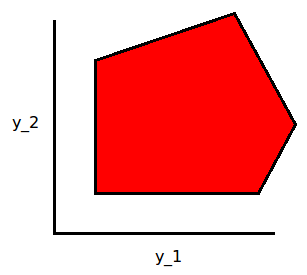
\includegraphics[width=8cm]{graph/sample_dos}
  \scalebox{1}{% Graphic for TeX using PGF
% Title: /home/andre/GIT Repos/AHCampher_thesis/diagrams/sampledos.dia
% Creator: Dia v0.97.1
% CreationDate: Thu Jan  6 14:33:46 2011
% For: andre
% \usepackage{tikz}
% The following commands are not supported in PSTricks at present
% We define them conditionally, so when they are implemented,
% this pgf file will use them.
\ifx\du\undefined
  \newlength{\du}
\fi
\setlength{\du}{15\unitlength}
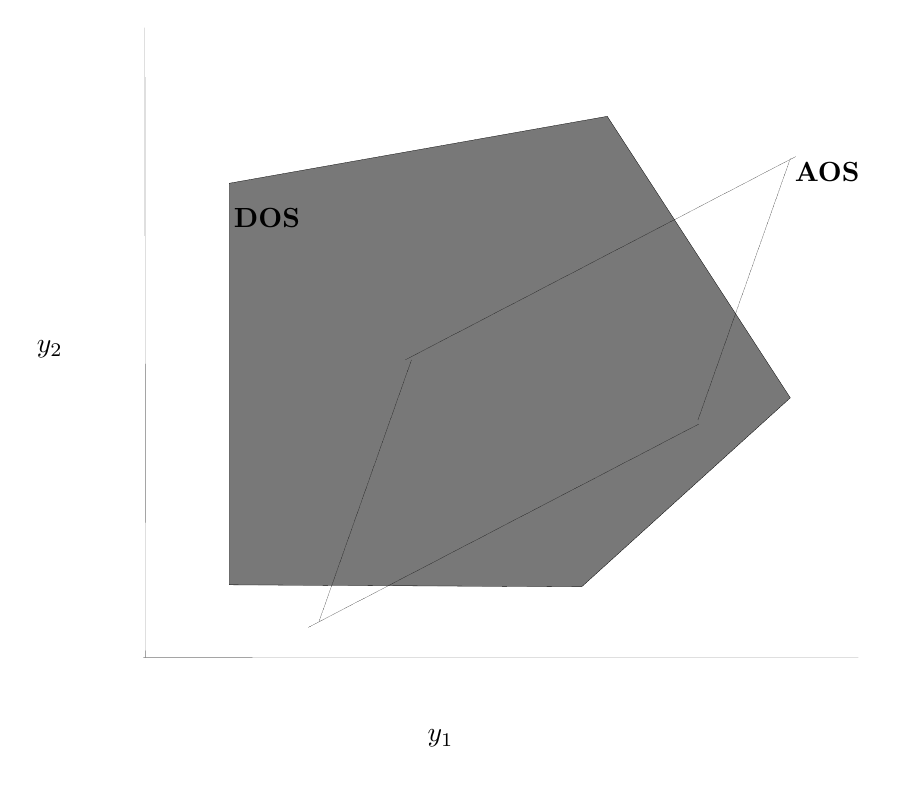
\begin{tikzpicture}
\pgftransformxscale{1.000000}
\pgftransformyscale{-1.000000}
\definecolor{dialinecolor}{rgb}{0.000000, 0.000000, 0.000000}
\pgfsetstrokecolor{dialinecolor}
\definecolor{dialinecolor}{rgb}{1.000000, 1.000000, 1.000000}
\pgfsetfillcolor{dialinecolor}
\pgfsetlinewidth{0.050000\du}
\pgfsetdash{}{0pt}
\pgfsetdash{}{0pt}
\pgfsetbuttcap
{
\definecolor{dialinecolor}{rgb}{0.000000, 0.000000, 0.000000}
\pgfsetfillcolor{dialinecolor}
% was here!!!
\definecolor{dialinecolor}{rgb}{0.000000, 0.000000, 0.000000}
\pgfsetstrokecolor{dialinecolor}
\draw (0.511161\du,2.996885\du)--(0.518134\du,10.993760\du);
}
\pgfsetlinewidth{0.050000\du}
\pgfsetdash{}{0pt}
\pgfsetdash{}{0pt}
\pgfsetbuttcap
{
\definecolor{dialinecolor}{rgb}{0.000000, 0.000000, 0.000000}
\pgfsetfillcolor{dialinecolor}
% was here!!!
\definecolor{dialinecolor}{rgb}{0.000000, 0.000000, 0.000000}
\pgfsetstrokecolor{dialinecolor}
\draw (9.573661\du,10.996885\du)--(0.492855\du,10.995323\du);
}
% setfont left to latex
\definecolor{dialinecolor}{rgb}{0.000000, 0.000000, 0.000000}
\pgfsetstrokecolor{dialinecolor}
\node[anchor=west] at (-0.978316\du,7.075781\du){$y_2$};
% setfont left to latex
\definecolor{dialinecolor}{rgb}{0.000000, 0.000000, 0.000000}
\pgfsetstrokecolor{dialinecolor}
\node[anchor=west] at (3.984184\du,12.025781\du){$y_1$};
\pgfsetlinewidth{0.100000\du}
\pgfsetdash{}{0pt}
\pgfsetdash{}{0pt}
\pgfsetmiterjoin
\pgfsetbuttcap
\definecolor{dialinecolor}{rgb}{0.470588, 0.470588, 0.470588}
\pgfsetfillcolor{dialinecolor}
\fill (1.582934\du,10.071885\du)--(6.057934\du,10.096885\du)--(8.707934\du,7.696885\du)--(6.382934\du,4.121885\du)--(1.582934\du,4.971885\du)--cycle;
\definecolor{dialinecolor}{rgb}{0.000000, 0.000000, 0.000000}
\pgfsetstrokecolor{dialinecolor}
\draw (1.582934\du,10.071885\du)--(6.057934\du,10.096885\du)--(8.707934\du,7.696885\du)--(6.382934\du,4.121885\du)--(1.582934\du,4.971885\du)--cycle;
\pgfsetlinewidth{0.100000\du}
\pgfsetdash{{0.200000\du}{0.200000\du}}{0\du}
\pgfsetdash{{0.200000\du}{0.200000\du}}{0\du}
\pgfsetbuttcap
{
\definecolor{dialinecolor}{rgb}{0.000000, 0.000000, 0.000000}
\pgfsetfillcolor{dialinecolor}
% was here!!!
\definecolor{dialinecolor}{rgb}{0.000000, 0.000000, 0.000000}
\pgfsetstrokecolor{dialinecolor}
\draw (8.773661\du,4.634385\du)--(3.820050\du,7.213487\du);
}
\pgfsetlinewidth{0.100000\du}
\pgfsetdash{{0.200000\du}{0.200000\du}}{0\du}
\pgfsetdash{{0.200000\du}{0.200000\du}}{0\du}
\pgfsetbuttcap
{
\definecolor{dialinecolor}{rgb}{0.000000, 0.000000, 0.000000}
\pgfsetfillcolor{dialinecolor}
% was here!!!
\definecolor{dialinecolor}{rgb}{0.000000, 0.000000, 0.000000}
\pgfsetstrokecolor{dialinecolor}
\draw (7.542211\du,8.031824\du)--(2.588600\du,10.610926\du);
}
\pgfsetlinewidth{0.100000\du}
\pgfsetdash{{0.200000\du}{0.200000\du}}{0\du}
\pgfsetdash{{0.200000\du}{0.200000\du}}{0\du}
\pgfsetbuttcap
{
\definecolor{dialinecolor}{rgb}{0.000000, 0.000000, 0.000000}
\pgfsetfillcolor{dialinecolor}
% was here!!!
\definecolor{dialinecolor}{rgb}{0.000000, 0.000000, 0.000000}
\pgfsetstrokecolor{dialinecolor}
\draw (2.723661\du,10.534385\du)--(3.898661\du,7.209385\du);
}
\pgfsetlinewidth{0.100000\du}
\pgfsetdash{{0.200000\du}{0.200000\du}}{0\du}
\pgfsetdash{{0.200000\du}{0.200000\du}}{0\du}
\pgfsetbuttcap
{
\definecolor{dialinecolor}{rgb}{0.000000, 0.000000, 0.000000}
\pgfsetfillcolor{dialinecolor}
% was here!!!
\definecolor{dialinecolor}{rgb}{0.000000, 0.000000, 0.000000}
\pgfsetstrokecolor{dialinecolor}
\draw (7.534963\du,7.978188\du)--(8.709963\du,4.653188\du);
}
% setfont left to latex
\definecolor{dialinecolor}{rgb}{0.000000, 0.000000, 0.000000}
\pgfsetstrokecolor{dialinecolor}
\node[anchor=west] at (1.523661\du,5.409385\du){{\bf DOS}};
% setfont left to latex
\definecolor{dialinecolor}{rgb}{0.000000, 0.000000, 0.000000}
\pgfsetstrokecolor{dialinecolor}
\node[anchor=west] at (8.646161\du,4.834385\du){{\bf AOS}};
\end{tikzpicture}
}
  \caption[Sample Desired Output Space]{Sample Desired Output Space (DOS, with linear constraints on both outputs) along with a linear AOS}
  \label{fig:sampledos}
\end{figure}

\begin{figure}[htbp]
  \centering
%  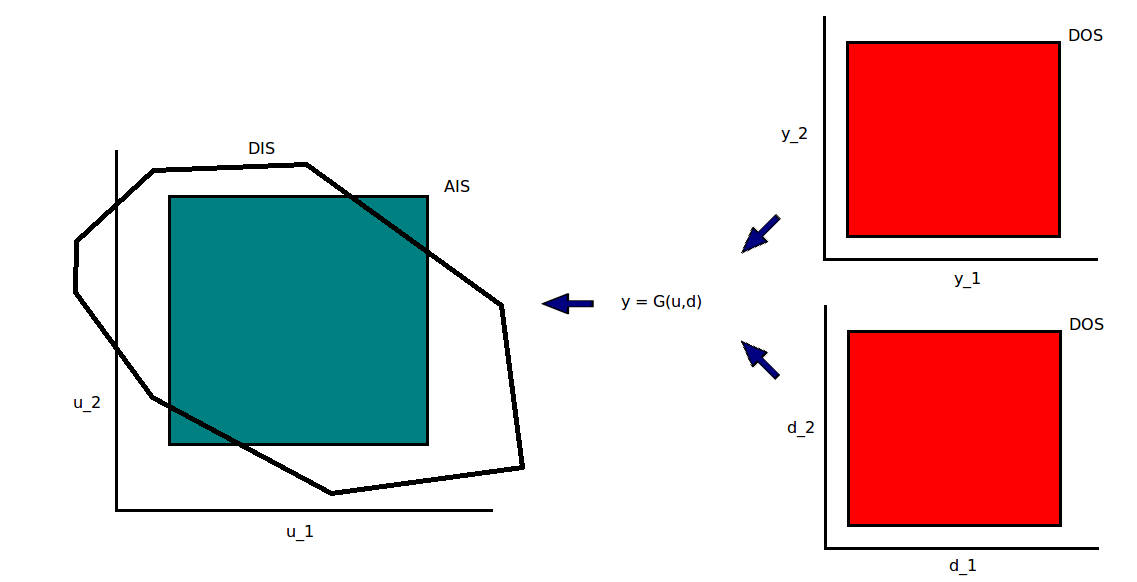
\includegraphics[width=\fullwidth]{graph/sample_dis}
  \scalebox{1}{% Graphic for TeX using PGF
% Title: /home/andre/GIT Repos/AHCampher_thesis/diagrams/sampledis.dia
% Creator: Dia v0.97.1
% CreationDate: Thu Jan  6 14:49:42 2011
% For: andre
% \usepackage{tikz}
% The following commands are not supported in PSTricks at present
% We define them conditionally, so when they are implemented,
% this pgf file will use them.
\ifx\du\undefined
  \newlength{\du}
\fi
\setlength{\du}{15\unitlength}
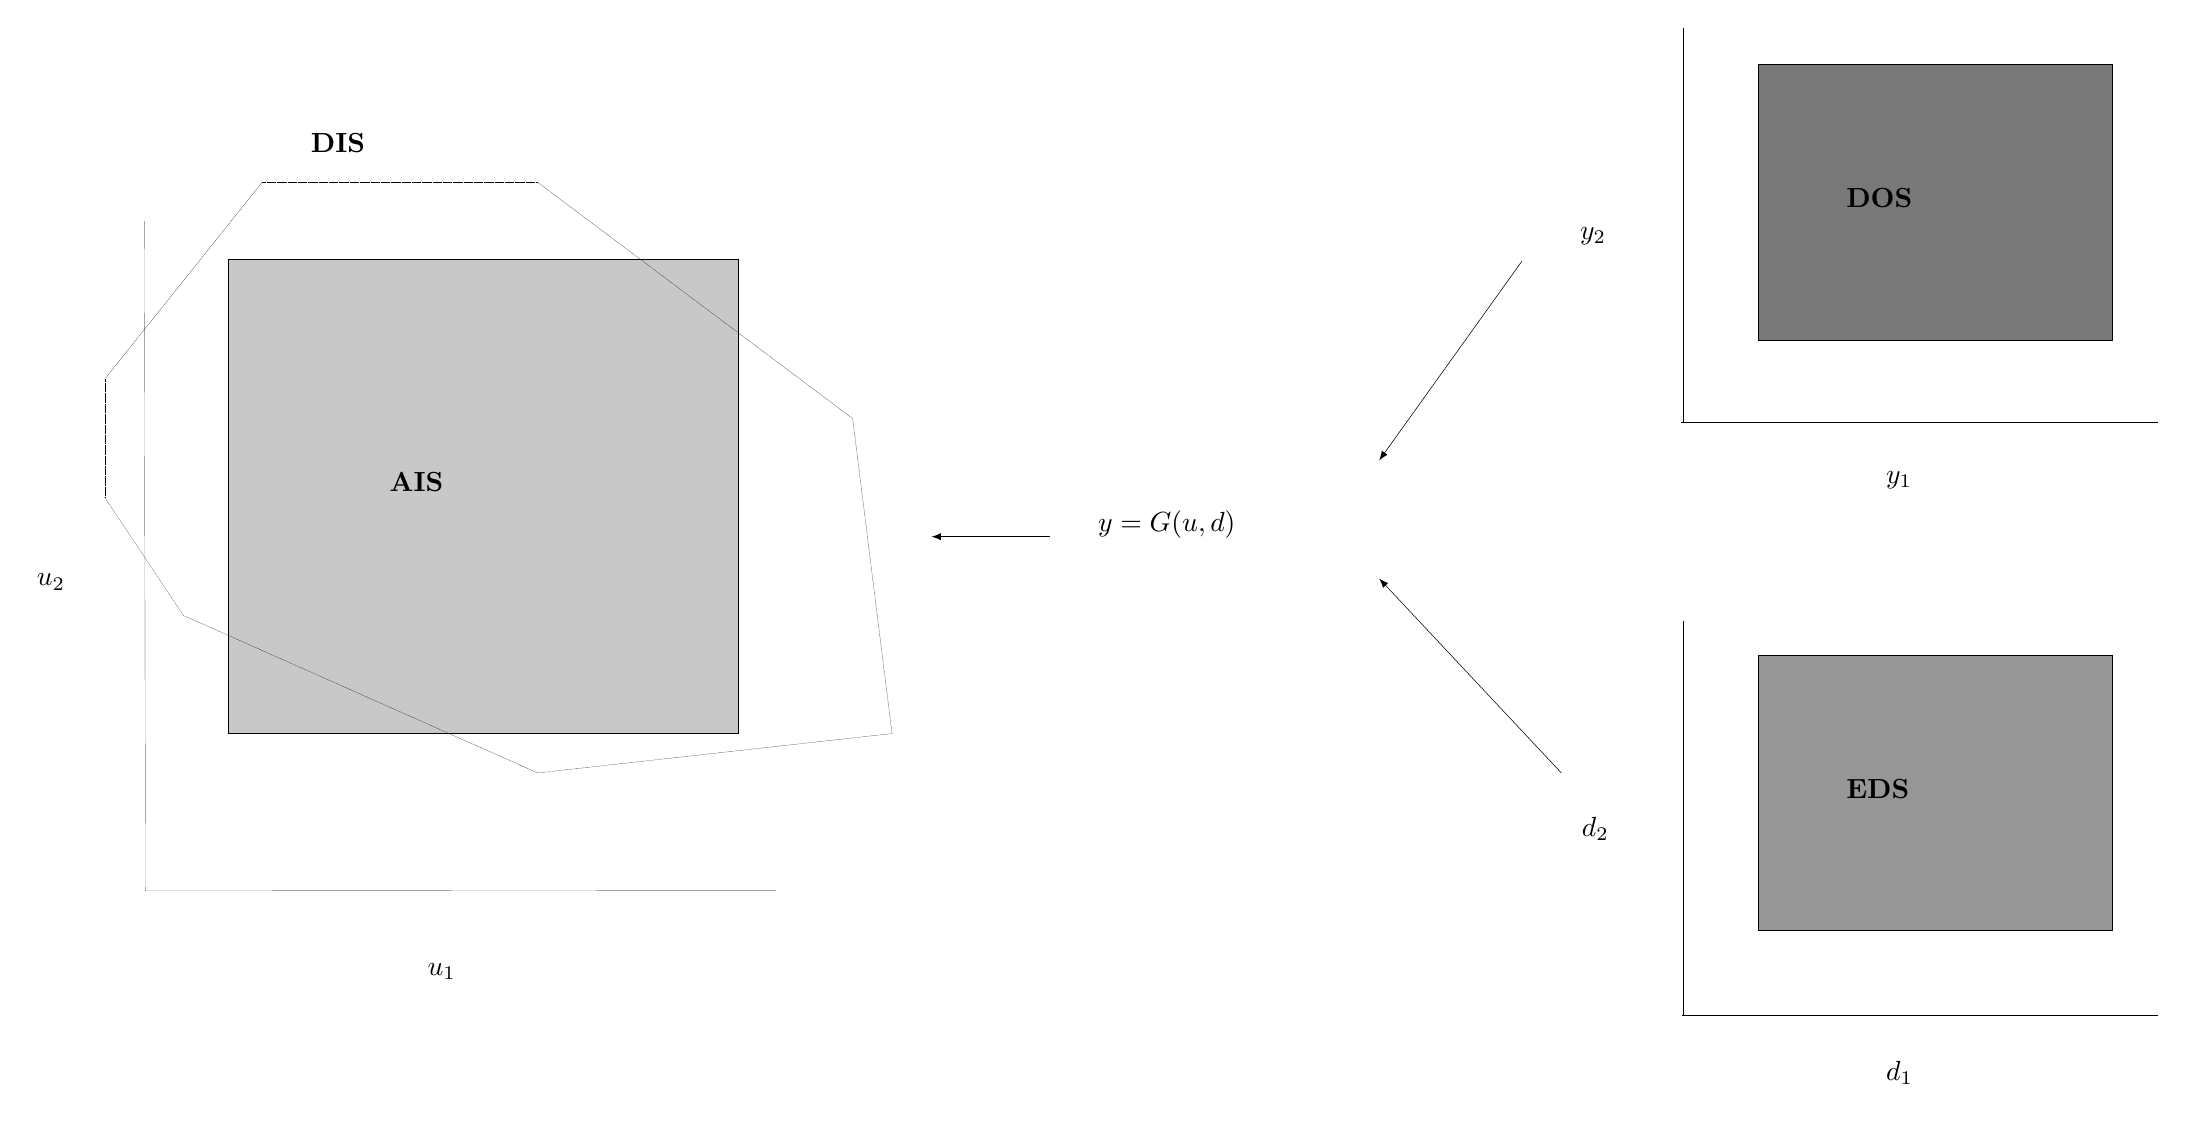
\begin{tikzpicture}
\pgftransformxscale{1.000000}
\pgftransformyscale{-1.000000}
\definecolor{dialinecolor}{rgb}{0.000000, 0.000000, 0.000000}
\pgfsetstrokecolor{dialinecolor}
\definecolor{dialinecolor}{rgb}{1.000000, 1.000000, 1.000000}
\pgfsetfillcolor{dialinecolor}
\pgfsetlinewidth{0.100000\du}
\pgfsetdash{}{0pt}
\pgfsetdash{}{0pt}
\pgfsetmiterjoin
\definecolor{dialinecolor}{rgb}{0.784314, 0.784314, 0.784314}
\pgfsetfillcolor{dialinecolor}
\fill (1.574380\du,2.981260\du)--(1.574380\du,9.000000\du)--(8.047071\du,9.000000\du)--(8.047071\du,2.981260\du)--cycle;
\definecolor{dialinecolor}{rgb}{0.000000, 0.000000, 0.000000}
\pgfsetstrokecolor{dialinecolor}
\draw (1.574380\du,2.981260\du)--(1.574380\du,9.000000\du)--(8.047071\du,9.000000\du)--(8.047071\du,2.981260\du)--cycle;
\pgfsetlinewidth{0.050000\du}
\pgfsetdash{}{0pt}
\pgfsetdash{}{0pt}
\pgfsetbuttcap
{
\definecolor{dialinecolor}{rgb}{0.000000, 0.000000, 0.000000}
\pgfsetfillcolor{dialinecolor}
% was here!!!
\definecolor{dialinecolor}{rgb}{0.000000, 0.000000, 0.000000}
\pgfsetstrokecolor{dialinecolor}
\draw (0.503325\du,2.493750\du)--(0.518134\du,10.993800\du);
}
\pgfsetlinewidth{0.050000\du}
\pgfsetdash{}{0pt}
\pgfsetdash{}{0pt}
\pgfsetbuttcap
{
\definecolor{dialinecolor}{rgb}{0.000000, 0.000000, 0.000000}
\pgfsetfillcolor{dialinecolor}
% was here!!!
\definecolor{dialinecolor}{rgb}{0.000000, 0.000000, 0.000000}
\pgfsetstrokecolor{dialinecolor}
\draw (8.525170\du,10.989100\du)--(0.492855\du,10.995300\du);
}
% setfont left to latex
\definecolor{dialinecolor}{rgb}{0.000000, 0.000000, 0.000000}
\pgfsetstrokecolor{dialinecolor}
\node[anchor=west] at (-0.978316\du,7.075780\du){$u_2$};
% setfont left to latex
\definecolor{dialinecolor}{rgb}{0.000000, 0.000000, 0.000000}
\pgfsetstrokecolor{dialinecolor}
\node[anchor=west] at (3.984180\du,12.025800\du){$u_1$};
\pgfsetlinewidth{0.050000\du}
\pgfsetdash{}{0pt}
\pgfsetdash{}{0pt}
\pgfsetbuttcap
{
\definecolor{dialinecolor}{rgb}{0.000000, 0.000000, 0.000000}
\pgfsetfillcolor{dialinecolor}
% was here!!!
\definecolor{dialinecolor}{rgb}{0.000000, 0.000000, 0.000000}
\pgfsetstrokecolor{dialinecolor}
\draw (20.050800\du,0.036250\du)--(20.050800\du,5.061250\du);
}
\pgfsetlinewidth{0.050000\du}
\pgfsetdash{}{0pt}
\pgfsetdash{}{0pt}
\pgfsetbuttcap
{
\definecolor{dialinecolor}{rgb}{0.000000, 0.000000, 0.000000}
\pgfsetfillcolor{dialinecolor}
% was here!!!
\definecolor{dialinecolor}{rgb}{0.000000, 0.000000, 0.000000}
\pgfsetstrokecolor{dialinecolor}
\draw (26.075800\du,5.048750\du)--(20.025800\du,5.048750\du);
}
% setfont left to latex
\definecolor{dialinecolor}{rgb}{0.000000, 0.000000, 0.000000}
\pgfsetstrokecolor{dialinecolor}
\node[anchor=west] at (18.619200\du,2.680780\du){$y_2$};
% setfont left to latex
\definecolor{dialinecolor}{rgb}{0.000000, 0.000000, 0.000000}
\pgfsetstrokecolor{dialinecolor}
\node[anchor=west] at (22.506700\du,5.780780\du){$y_1$};
\pgfsetlinewidth{0.050000\du}
\pgfsetdash{}{0pt}
\pgfsetdash{}{0pt}
\pgfsetbuttcap
{
\definecolor{dialinecolor}{rgb}{0.000000, 0.000000, 0.000000}
\pgfsetfillcolor{dialinecolor}
% was here!!!
\definecolor{dialinecolor}{rgb}{0.000000, 0.000000, 0.000000}
\pgfsetstrokecolor{dialinecolor}
\draw (20.050900\du,7.566260\du)--(20.050900\du,12.591300\du);
}
\pgfsetlinewidth{0.050000\du}
\pgfsetdash{}{0pt}
\pgfsetdash{}{0pt}
\pgfsetbuttcap
{
\definecolor{dialinecolor}{rgb}{0.000000, 0.000000, 0.000000}
\pgfsetfillcolor{dialinecolor}
% was here!!!
\definecolor{dialinecolor}{rgb}{0.000000, 0.000000, 0.000000}
\pgfsetstrokecolor{dialinecolor}
\draw (26.075900\du,12.578800\du)--(20.025900\du,12.578800\du);
}
% setfont left to latex
\definecolor{dialinecolor}{rgb}{0.000000, 0.000000, 0.000000}
\pgfsetstrokecolor{dialinecolor}
\node[anchor=west] at (18.644300\du,10.210800\du){$d_2$};
% setfont left to latex
\definecolor{dialinecolor}{rgb}{0.000000, 0.000000, 0.000000}
\pgfsetstrokecolor{dialinecolor}
\node[anchor=west] at (22.506800\du,13.310800\du){$d_1$};
% setfont left to latex
\definecolor{dialinecolor}{rgb}{0.000000, 0.000000, 0.000000}
\pgfsetstrokecolor{dialinecolor}
\node[anchor=west] at (12.500000\du,6.3500000\du){$y = G(\vect{u},\vect{d})$};
\pgfsetlinewidth{0.200000\du}
\pgfsetdash{}{0pt}
\pgfsetdash{}{0pt}
\pgfsetbuttcap
{
\definecolor{dialinecolor}{rgb}{0.000000, 0.000000, 0.000000}
\pgfsetfillcolor{dialinecolor}
% was here!!!
\pgfsetarrowsend{latex}
\definecolor{dialinecolor}{rgb}{0.000000, 0.000000, 0.000000}
\pgfsetstrokecolor{dialinecolor}
\draw (12.000000\du,6.500000\du)--(10.500000\du,6.500000\du);
}
\pgfsetlinewidth{0.200000\du}
\pgfsetdash{}{0pt}
\pgfsetdash{}{0pt}
\pgfsetbuttcap
{
\definecolor{dialinecolor}{rgb}{0.000000, 0.000000, 0.000000}
\pgfsetfillcolor{dialinecolor}
% was here!!!
\pgfsetarrowsend{latex}
\definecolor{dialinecolor}{rgb}{0.000000, 0.000000, 0.000000}
\pgfsetstrokecolor{dialinecolor}
\draw (18.000000\du,3.000000\du)--(16.186200\du,5.531370\du);
}
\pgfsetlinewidth{0.200000\du}
\pgfsetdash{}{0pt}
\pgfsetdash{}{0pt}
\pgfsetbuttcap
{
\definecolor{dialinecolor}{rgb}{0.000000, 0.000000, 0.000000}
\pgfsetfillcolor{dialinecolor}
% was here!!!
\pgfsetarrowsend{latex}
\definecolor{dialinecolor}{rgb}{0.000000, 0.000000, 0.000000}
\pgfsetstrokecolor{dialinecolor}
\draw (18.500000\du,9.500000\du)--(16.186100\du,7.031420\du);
}
\pgfsetlinewidth{0.100000\du}
\pgfsetdash{}{0pt}
\pgfsetdash{}{0pt}
\pgfsetmiterjoin
\definecolor{dialinecolor}{rgb}{0.470588, 0.470588, 0.470588}
\pgfsetfillcolor{dialinecolor}
\fill (21.000000\du,0.500000\du)--(21.000000\du,4.000000\du)--(25.500000\du,4.000000\du)--(25.500000\du,0.500000\du)--cycle;
\definecolor{dialinecolor}{rgb}{0.000000, 0.000000, 0.000000}
\pgfsetstrokecolor{dialinecolor}
\draw (21.000000\du,0.500000\du)--(21.000000\du,4.000000\du)--(25.500000\du,4.000000\du)--(25.500000\du,0.500000\du)--cycle;
\pgfsetlinewidth{0.100000\du}
\pgfsetdash{}{0pt}
\pgfsetdash{}{0pt}
\pgfsetmiterjoin
\definecolor{dialinecolor}{rgb}{0.588235, 0.588235, 0.588235}
\pgfsetfillcolor{dialinecolor}
\fill (21.000000\du,8.000000\du)--(21.000000\du,11.500000\du)--(25.500000\du,11.500000\du)--(25.500000\du,8.000000\du)--cycle;
\definecolor{dialinecolor}{rgb}{0.000000, 0.000000, 0.000000}
\pgfsetstrokecolor{dialinecolor}
\draw (21.000000\du,8.000000\du)--(21.000000\du,11.500000\du)--(25.500000\du,11.500000\du)--(25.500000\du,8.000000\du)--cycle;
% setfont left to latex
\definecolor{dialinecolor}{rgb}{0.000000, 0.000000, 0.000000}
\pgfsetstrokecolor{dialinecolor}
\node[anchor=west] at (22.000000\du,2.200000\du){\bf DOS};
% setfont left to latex
\definecolor{dialinecolor}{rgb}{0.000000, 0.000000, 0.000000}
\pgfsetstrokecolor{dialinecolor}
\node[anchor=west] at (22.000000\du,9.700000\du){\bf EDS};
% setfont left to latex
\definecolor{dialinecolor}{rgb}{0.000000, 0.000000, 0.000000}
\pgfsetstrokecolor{dialinecolor}
\node[anchor=west] at (3.500000\du,5.800000\du){\bf AIS};
\pgfsetlinewidth{0.100000\du}
\pgfsetdash{{0.200000\du}{0.200000\du}}{0\du}
\pgfsetdash{{0.200000\du}{0.200000\du}}{0\du}
\pgfsetbuttcap
{
\definecolor{dialinecolor}{rgb}{0.000000, 0.000000, 0.000000}
\pgfsetfillcolor{dialinecolor}
% was here!!!
\definecolor{dialinecolor}{rgb}{0.000000, 0.000000, 0.000000}
\pgfsetstrokecolor{dialinecolor}
\draw (5.500000\du,2.000000\du)--(9.500000\du,5.000000\du);
}
\pgfsetlinewidth{0.100000\du}
\pgfsetdash{{0.200000\du}{0.200000\du}}{0\du}
\pgfsetdash{{0.200000\du}{0.200000\du}}{0\du}
\pgfsetbuttcap
{
\definecolor{dialinecolor}{rgb}{0.000000, 0.000000, 0.000000}
\pgfsetfillcolor{dialinecolor}
% was here!!!
\definecolor{dialinecolor}{rgb}{0.000000, 0.000000, 0.000000}
\pgfsetstrokecolor{dialinecolor}
\draw (2.000000\du,2.000000\du)--(5.500000\du,2.000000\du);
}
\pgfsetlinewidth{0.100000\du}
\pgfsetdash{{0.200000\du}{0.200000\du}}{0\du}
\pgfsetdash{{0.200000\du}{0.200000\du}}{0\du}
\pgfsetbuttcap
{
\definecolor{dialinecolor}{rgb}{0.000000, 0.000000, 0.000000}
\pgfsetfillcolor{dialinecolor}
% was here!!!
\definecolor{dialinecolor}{rgb}{0.000000, 0.000000, 0.000000}
\pgfsetstrokecolor{dialinecolor}
\draw (2.000000\du,2.000000\du)--(0.000000\du,4.500000\du);
}
\pgfsetlinewidth{0.100000\du}
\pgfsetdash{{0.200000\du}{0.200000\du}}{0\du}
\pgfsetdash{{0.200000\du}{0.200000\du}}{0\du}
\pgfsetbuttcap
{
\definecolor{dialinecolor}{rgb}{0.000000, 0.000000, 0.000000}
\pgfsetfillcolor{dialinecolor}
% was here!!!
\definecolor{dialinecolor}{rgb}{0.000000, 0.000000, 0.000000}
\pgfsetstrokecolor{dialinecolor}
\draw (0.000000\du,4.500000\du)--(0.000000\du,6.000000\du);
}
\pgfsetlinewidth{0.100000\du}
\pgfsetdash{{0.200000\du}{0.200000\du}}{0\du}
\pgfsetdash{{0.200000\du}{0.200000\du}}{0\du}
\pgfsetbuttcap
{
\definecolor{dialinecolor}{rgb}{0.000000, 0.000000, 0.000000}
\pgfsetfillcolor{dialinecolor}
% was here!!!
\definecolor{dialinecolor}{rgb}{0.000000, 0.000000, 0.000000}
\pgfsetstrokecolor{dialinecolor}
\draw (0.000000\du,6.000000\du)--(1.000000\du,7.500000\du);
}
\pgfsetlinewidth{0.100000\du}
\pgfsetdash{{0.200000\du}{0.200000\du}}{0\du}
\pgfsetdash{{0.200000\du}{0.200000\du}}{0\du}
\pgfsetbuttcap
{
\definecolor{dialinecolor}{rgb}{0.000000, 0.000000, 0.000000}
\pgfsetfillcolor{dialinecolor}
% was here!!!
\definecolor{dialinecolor}{rgb}{0.000000, 0.000000, 0.000000}
\pgfsetstrokecolor{dialinecolor}
\draw (1.000000\du,7.500000\du)--(5.500000\du,9.500000\du);
}
\pgfsetlinewidth{0.100000\du}
\pgfsetdash{{0.200000\du}{0.200000\du}}{0\du}
\pgfsetdash{{0.200000\du}{0.200000\du}}{0\du}
\pgfsetbuttcap
{
\definecolor{dialinecolor}{rgb}{0.000000, 0.000000, 0.000000}
\pgfsetfillcolor{dialinecolor}
% was here!!!
\definecolor{dialinecolor}{rgb}{0.000000, 0.000000, 0.000000}
\pgfsetstrokecolor{dialinecolor}
\draw (9.500000\du,5.000000\du)--(10.000000\du,9.000000\du);
}
\pgfsetlinewidth{0.100000\du}
\pgfsetdash{{0.200000\du}{0.200000\du}}{0\du}
\pgfsetdash{{0.200000\du}{0.200000\du}}{0\du}
\pgfsetbuttcap
{
\definecolor{dialinecolor}{rgb}{0.000000, 0.000000, 0.000000}
\pgfsetfillcolor{dialinecolor}
% was here!!!
\definecolor{dialinecolor}{rgb}{0.000000, 0.000000, 0.000000}
\pgfsetstrokecolor{dialinecolor}
\draw (5.500000\du,9.500000\du)--(10.000000\du,9.000000\du);
}
% setfont left to latex
\definecolor{dialinecolor}{rgb}{0.000000, 0.000000, 0.000000}
\pgfsetstrokecolor{dialinecolor}
\node[anchor=west] at (2.500000\du,1.500000\du){\bf DIS};
\end{tikzpicture}
}
  \caption[Sample Desired Input Space]{Sample Desired Input Space (DIS) for
    a linear model and rectangular DOS and EDS}
  \label{fig:sampledis}
\end{figure}

\citet{vinsonphd} defines the generalised Output Operability Index (OOI\nomenclature[ba]{OOI}{Output Operability Index}) as shown in equation~\ref{eq:genooi}. 
From this definition it is clear that the operability of a process decreases if the AOS does not cover the whole DOS. 
Servo- and regulatory operability indices are also defined in the text, but are not shown here.
\begin{equation}
  \label{eq:genooi}
     OOI \triangleq \frac{\mu(AOS\cap DOS)}{\mu(DOS)}
\end{equation}
where $\mu$ represents a function to calculate the volume of a space.%
\nomenclature[ga]{$\mu$}{Volume of a polytope}%

All the concepts above are directly applicable to square systems.
For the case of non-square systems (more outputs than inputs) the Operability Index formulation is extended to interval operability. 
In this case, process outputs are split into two categories; setpoint controlled variables and range controlled variables.
The first being controlled on a given setpoint, whereas the later is allowed to vary within its given maximum and minimum limits.

\citet{limaphd} elaborates on the interval operability of linear non-square systems and defines the following spaces:
\begin{description}
  \item [The interval AOS (AOS$_I$);] which is the union of all AOS($d$) where $d$ is within the EDS. 
This is typically generated by the shifting of AOS($d=0$) in the directions determined by $G_d$ (the disturbance model).%
\nomenclature[ba]{AOS$_I$}{Interval AOS}%
  \item [The Achievable Output Interval Set (AOIS);] defined as a rectangle with the same aspect ratio as the DOS, bound by the lines (or hyperplanes) that correspond to the minimum and maximum values of $d$ in the AOS. 
Since the issue of interval operability is being addressed, the AOIS does not need to be strictly contained within the AOS$_I$.%
\nomenclature[ba]{AOIS}{Achievable Output Interval Set}%
\end{description}
\citet{limaphd} proceeds to define a hyper-volume ratio (HVR) as shown in equation~\ref{eq:hvr}. 
The aim being here to define a measure for obtaining tighter control on CVs by reducing the size of the DOS (without causing infeasibilities). 
The process remains interval controllable as long as the AOIS remains a subset of the DOS (AOIS$\subseteq$DOS).
\begin{equation}
  \label{eq:hvr}
    HVR = \frac{\mu(DOS)}{\mu(AOIS)}
\end{equation}
where $\mu$ represents a function to calculate the volume of a space.%
\nomenclature[ba]{CV}{Controlled variable}%
\nomenclature[ba]{MV}{Manipulated variable}%
\nomenclature[ba]{DV}{Disturbance variable}%

To change the relative importance (tightness of control) on variables, weights are imposed on the AOIS. 
This in turn affects the aspect ratio of the AOIS.

\citet{limaphd} proposes two methods to calculate an AOIS for higher dimensional systems; an iterative method and a method based on linear programming (LP). 
In both cases, this corresponds to the tightest set of output constraints which still render the system controllable. 
Both methods are briefly discussed below:
\begin{itemize}
  \item Iterative approach; this method relies on the use of computational geometry tools to calculate convex hulls and intersections. 
An AOIS is initially estimated and expanded until it intersects the extreme subsets of the AOS. 
The magnitude by which the AOIS is increased is calculated using the Secant and bisection method. 
The calculations contained in this method are computationally intensive and limit its use to systems of 8 dimensions and lower.
  \item LP approach; in this approach the constraints and objective function are reformulated as linear functions. 
The extreme subsets of the AOS are expressed as linear inequalities and objective function set up as to determine the common intersection point of the AOIS and a given extreme subset. 
The proposed LP approach overcomes the computational intensity of the iterative method and is suitable for on-line calculation of the AOIS.
\end{itemize}

\subsubsection{Application}
Numerous authors have illustrated the application of the Operability Index (OI). 
\citet{opconproc} focus on a general application of the OI, emphasising its ability to identify inoperable processes without the need to specify a controller structure. 
\citet{opidealrx} applies the OI to the design of ideal reactors. 

\subsection{Operability Index application to MPC}
Although the  Operability Index can be used with square or non-square, linear or non-linear models, its easiest application is to linear models. 
This is advantageous as most of the current MPCs use linear models \citep{vinsonphd}.
Table~\ref{tab:mpcoi} highlights some properties of MPCs which lend themselves to the  application of the Operability Index.%
\nomenclature[ba]{MPC}{Model Predictive Control(ler)}%
\begin{table}[htbp]
  \centering
  \caption[Application of the Operability Index to MPC]{Application of the
    Operability Index to MPC \citep{vinsonphd}}
  \label{tab:mpcoi}
    \begin{tabular}{p{6cm} p{9cm}}
      \toprule
      MPC property & Operability Index property \\
      \midrule
      Linear process models & Calculation of the relevant spaces (AOS and DIS) is usually fast.\\[1.3ex]
      Constraints on MVs and CVs & In the case of fixed constraints; the input and output constraints result in polytopes in both the input and output spaces. 
From these descriptions the framework of Operability Index can be directly applied.\\[1.3ex]
      Solution of MV and CV steady state targets  & Where an LP solver is used, the Operability Index can yield useful information about process characteristics.\\
      \bottomrule
    \end{tabular}
\end{table}

\citet{vinsonphd} presents a list of additional issues that limit the performance of MPCs (with specific attention to AspenTech's DMCplus$^{\copyright}$) and proposes methods (using the Operability Index) to solve these problems. 
These methods are indirectly applicable to the proposed constraint handling method of this document and are presented here for that reason. 

Processes with considerable noise cause targets to move with each controller execution.
Typical ways to avoid this are limiting MV stepsize or filtering CVs, both of which have a stabilizing effect but result in a more sluggish controller. 
These limits may also cause the controller to not reach optimum solutions.
Using the OI and the associated output spaces, the possible outputs of a (newly) limited input space are clearly shown.
    
Disturbances can cause CVs to violate their constraints. 
In some cases, the controller might give up on a constraint and continue (now using a subset of the CVs).
Possible solutions include; model re-identification (in the case of an inconsistency), fixing the source of the disturbance or adding a DV to account for the disturbance.
Due to the fixed constraints on MVs and CVs the resulting AIS and DOS can be used to calculate the controller's ability to reject a disturbance. 
A measure of controller robustness can be derived from this.
    
Lastly, move suppression factors for MVs and give-ups for CVs are used to tune MPCs for dynamic performance.
The choice of these factors are usually qualitative and according to guidelines (and validated via offline simulations).
The OI (and its associated spaces) can provide guidance in determining move suppression factors and give-ups. 
The difficulty in controlling a CV at a given constraint can be derived from the OI.
How far a CV constraint can be moved (given the MV constraints) can also be determined from the OI.

% Local Variables:
% TeX-master: "AHC_thesis"
% End:
